\documentclass[11pt,letterpaper]{article}

% ============================================
% PACKAGES
% ============================================

% Page layout
\usepackage[margin=1in]{geometry}
\usepackage{setspace}
\usepackage{microtype}

% Figures and tables
\usepackage{graphicx}
\usepackage{float}
\usepackage{booktabs}
\usepackage{caption}
\usepackage{subcaption}


% Mathematics and scientific notation
\usepackage{amsmath}
\usepackage{amssymb}
\usepackage{siunitx}

% Bibliography (Zotero / BibLaTeX)
\usepackage[
    backend=biber,
    style=authoryear,
    sorting=nyt
]{biblatex}
\addbibresource{references.bib} % Change to your linked Zotero .bib filename if needed

% Hyperlinks and references
\usepackage[
    colorlinks=true,
    linkcolor=blue,
    citecolor=blue,
    urlcolor=blue
]{hyperref}

% After adding references to references.bib, cite with:
% \parencite{yourCitationKey} -- parenthetical citation
% \textcite{yourCitationKey}  -- author in the sentence

% ============================================
% DOCUMENT INFORMATION
% ============================================

\title{Denali Ice Cores Basal ECM Results}
\author{Liam Kirkpatrick, T.J. Fudge \\ University of Washington, Department of Earth Science}
\date{November 4, 2026}

\begin{document}

\maketitle

% ============================================
% ABSTRACT (OPTIONAL)
% ============================================

\begin{abstract}
This report summarizes results from 2D ECM measurements on the basal portion of the Denali ice cores. The goal of this work was to characterize the layering in this deepest ice, to evaluate the possibility of folding or disturbed stratigraphy. We find no visible evidence of folding in the clearly resolved layers. Apparent dip magnitudes are below $20^\circ$ for 29 of 30 fitted features; the one steeper estimate may reflect inconsistent tracking across a broad layer. These observations support preserved layering in the measured portions of DEN13A down to approximately 209.14 m, but do not establish continuous stratigraphy or constrain true dip from above.
\end{abstract}

% ============================================
\section{Methods}
% ============================================

\subsection{2D ECM measurements}

The ECM device setup in this study follows \textcite{kirkpatrick_three-dimensional_2025}. The AC ECM electrodes and overall device design are identical to the configuration described in this manuscript. However, in this study, ECM measurements are made on a single face (2D ECM), as in \textcite{fudge_electrical_2016}, rather than on two faces (3D ECM), as in \textcite{kirkpatrick_three-dimensional_2025}. We measured a total of 16 sections of the DEN13A core, with approximately 6.66 m of ice measured between 196.93 m and 211.02 m depth. Here, a section denotes one measured sample identifier (for example, 214abcdefg); some contain multiple core pieces. The total measured length is the sum of the depth spans of the 16 cleaned AC datasets, before plotting trims, and includes flagged intervals within those spans. Sampling is discontinuous across this depth range.

The DC electrodes applied in this study were experimental, and there are no other publications which describe these experimental electrodes in operation. We were not able to obtain DC ECM measurements on many of the sections in this study, due to time constraints and difficulties with the novel configuration. Additionally, we find that the DC ECM data is more noisy than the AC ECM data. We include a set of DC ECM figures in this report, but suggest that a final publication only includes the AC ECM data, for simplicity and because these are the clearest results. Without significant data shallower in the core or on other cores, interpreting the DC ECM data presented here is difficult. The use of AC ECM for layer orientation characterization follows other recent work with this instrument \parencite{kirkpatrick_three-dimensional_2025}.

\subsection{Apparent Dip calculation}

We manually selected depth windows containing recognizable AC ECM peaks or troughs. Within each window, we selected the depth of the raw maximum (peak) or minimum (trough) on every lateral track; tied extrema were assigned to the shallowest sample. We then fit an ordinary least-squares line, $z=a+bx$, to the picked depths $z$ and lateral positions $x$, expressed in the same units. The signed apparent dip is $\delta_{\mathrm{app}}=\arctan(b)$, positive where depth increases with increasing lateral position. Fits use all track picks, without smoothing, flag-based exclusions, outlier removal, or an imposed angle limit. The saved analysis contains 30 fitted features across nine sections, using 10 or 11 tracks per fit.

The plotted 95\% confidence intervals are Student-$t$ intervals for the fitted slope, transformed to angle. They quantify regression uncertainty conditional on the selected extrema; they do not include uncertainty from identifying the same layer across tracks, sample orientation, or systematic depth errors. Smoothing and normalization of the underlying color maps are for display only and do not affect the extrema used in the fits.

Apparent dip is the inclination seen on the measured face, whereas true dip is the maximum inclination of the layer plane. For a face parallel to the core axis, $\tan|\delta_{\mathrm{app}}|=\tan\delta_{\mathrm{true}}|\cos\phi|$, where $\phi$ is the angle between the face direction and the true dip direction \parencite{kirkpatrick_three-dimensional_2025}. Thus, apparent dip magnitude provides a lower bound on true dip, not an upper bound. A single face cannot determine true dip or its direction, and small apparent dips do not rule out steeper layers oriented obliquely to that face.


% ============================================
\section{Results}
% ============================================

We include examples from three sets of section figures. The first set shows AC ECM alone (Fig.~\ref{fig:AC_only_example}), with depth increasing downward and lateral track position on the horizontal axis. Color represents measured current in amperes. For display, the two outer tracks are normalized to the mean of the inner tracks, track ends are trimmed by 10 mm, and a 10 mm median smoothing window is applied. Each panel uses its own 5th--95th percentile color limits from unflagged, trimmed data, so colors should not be compared quantitatively between sections. Overlays identify surface imperfections, tephra or layers, rock or debris, and core breaks. These AC-only figures provide the clearest view for assessing lateral layer continuity.

\begin{figure}[H]
    \centering
    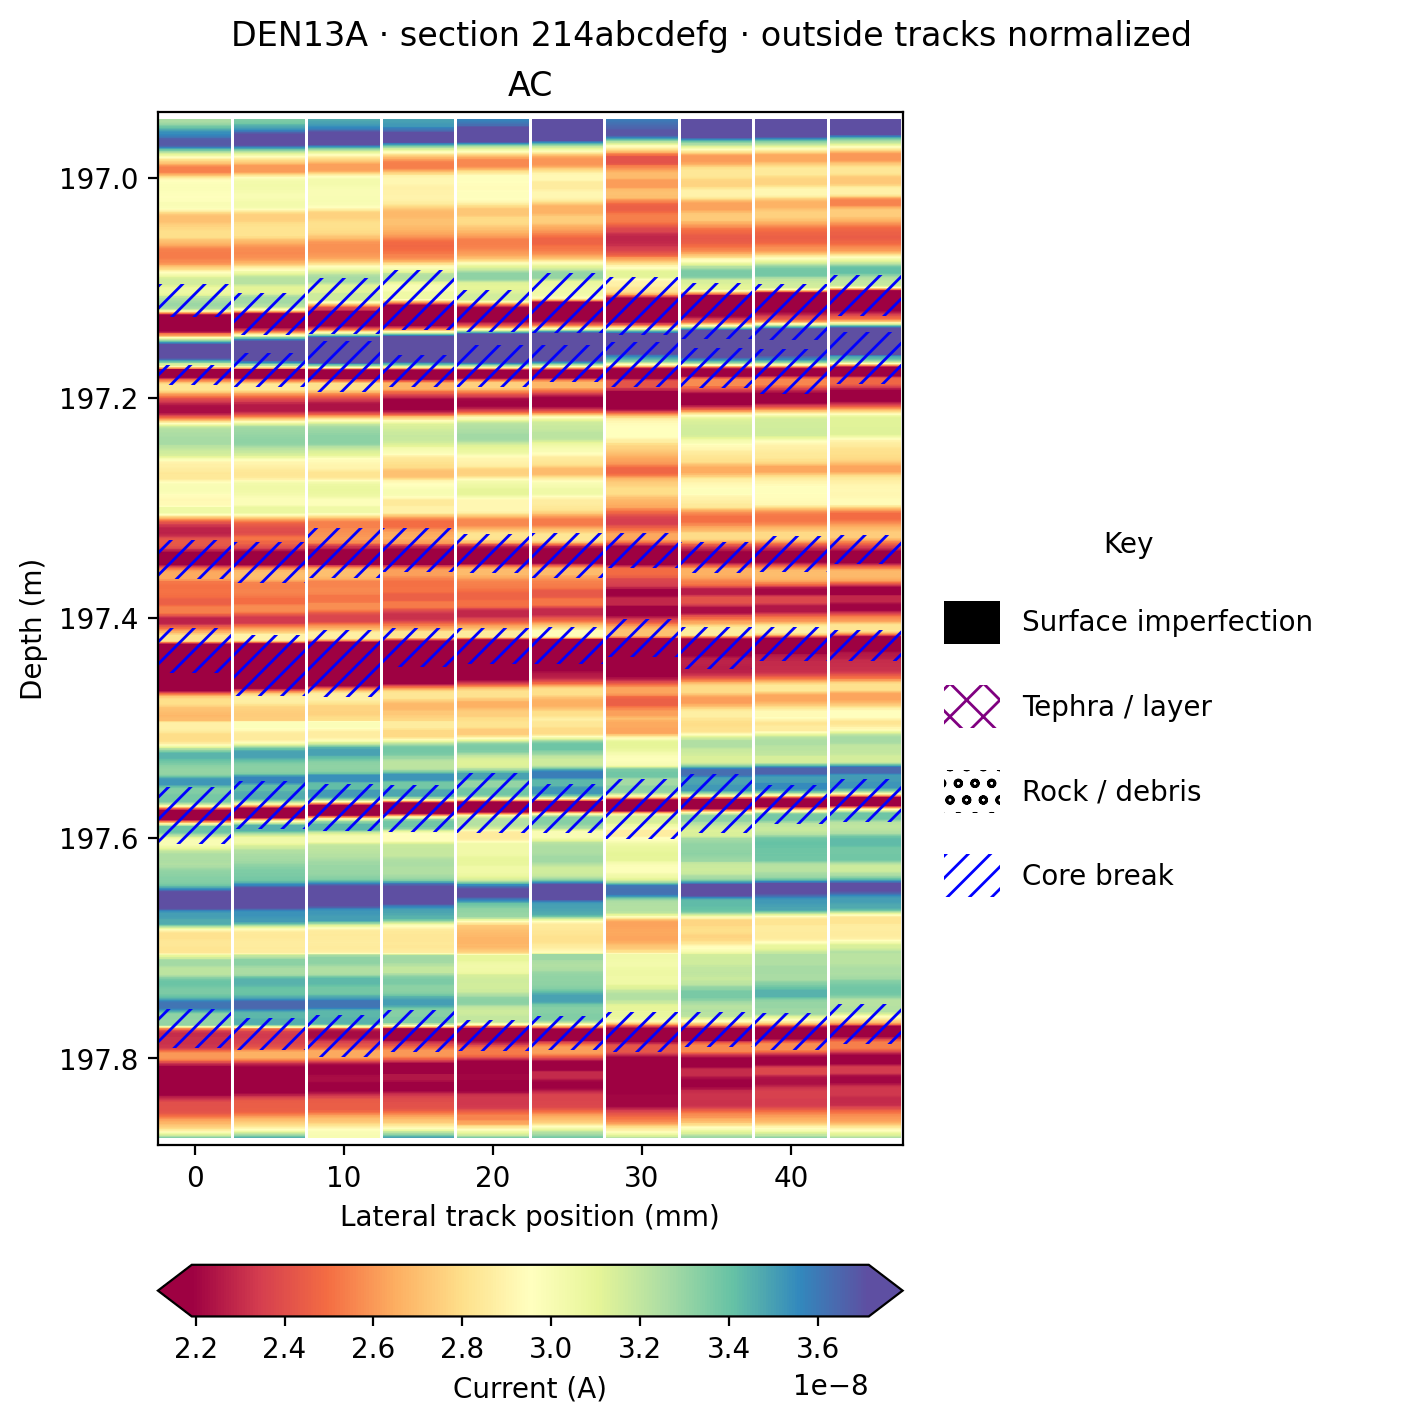
\includegraphics[width=0.72\textwidth]{figures/DEN13A-214abcdefg-AC-only.png}
    \caption{AC ECM for section 214abcdefg of DEN13A, illustrating well-defined bands that can be followed across the measured face. Color indicates current after outer-track normalization and display smoothing; blue diagonal hatching marks core breaks. Depth increases downward.}
    \label{fig:AC_only_example}
\end{figure}

Section 228d, extending to approximately 209.14 m in the trimmed AC map, is the deepest measured section in which we can clearly identify layering. Below this, the patterns are less clearly resolved and more difficult to interpret. Section 230a (Fig.~\ref{fig:AC_unclear_example}) illustrates this limitation: broad changes in current are visible, but distinct, well-defined layers are not readily traceable. The absence of clear layering in these deeper sections does not by itself demonstrate folding or stratigraphic disruption.

\begin{figure}[H]
    \centering
    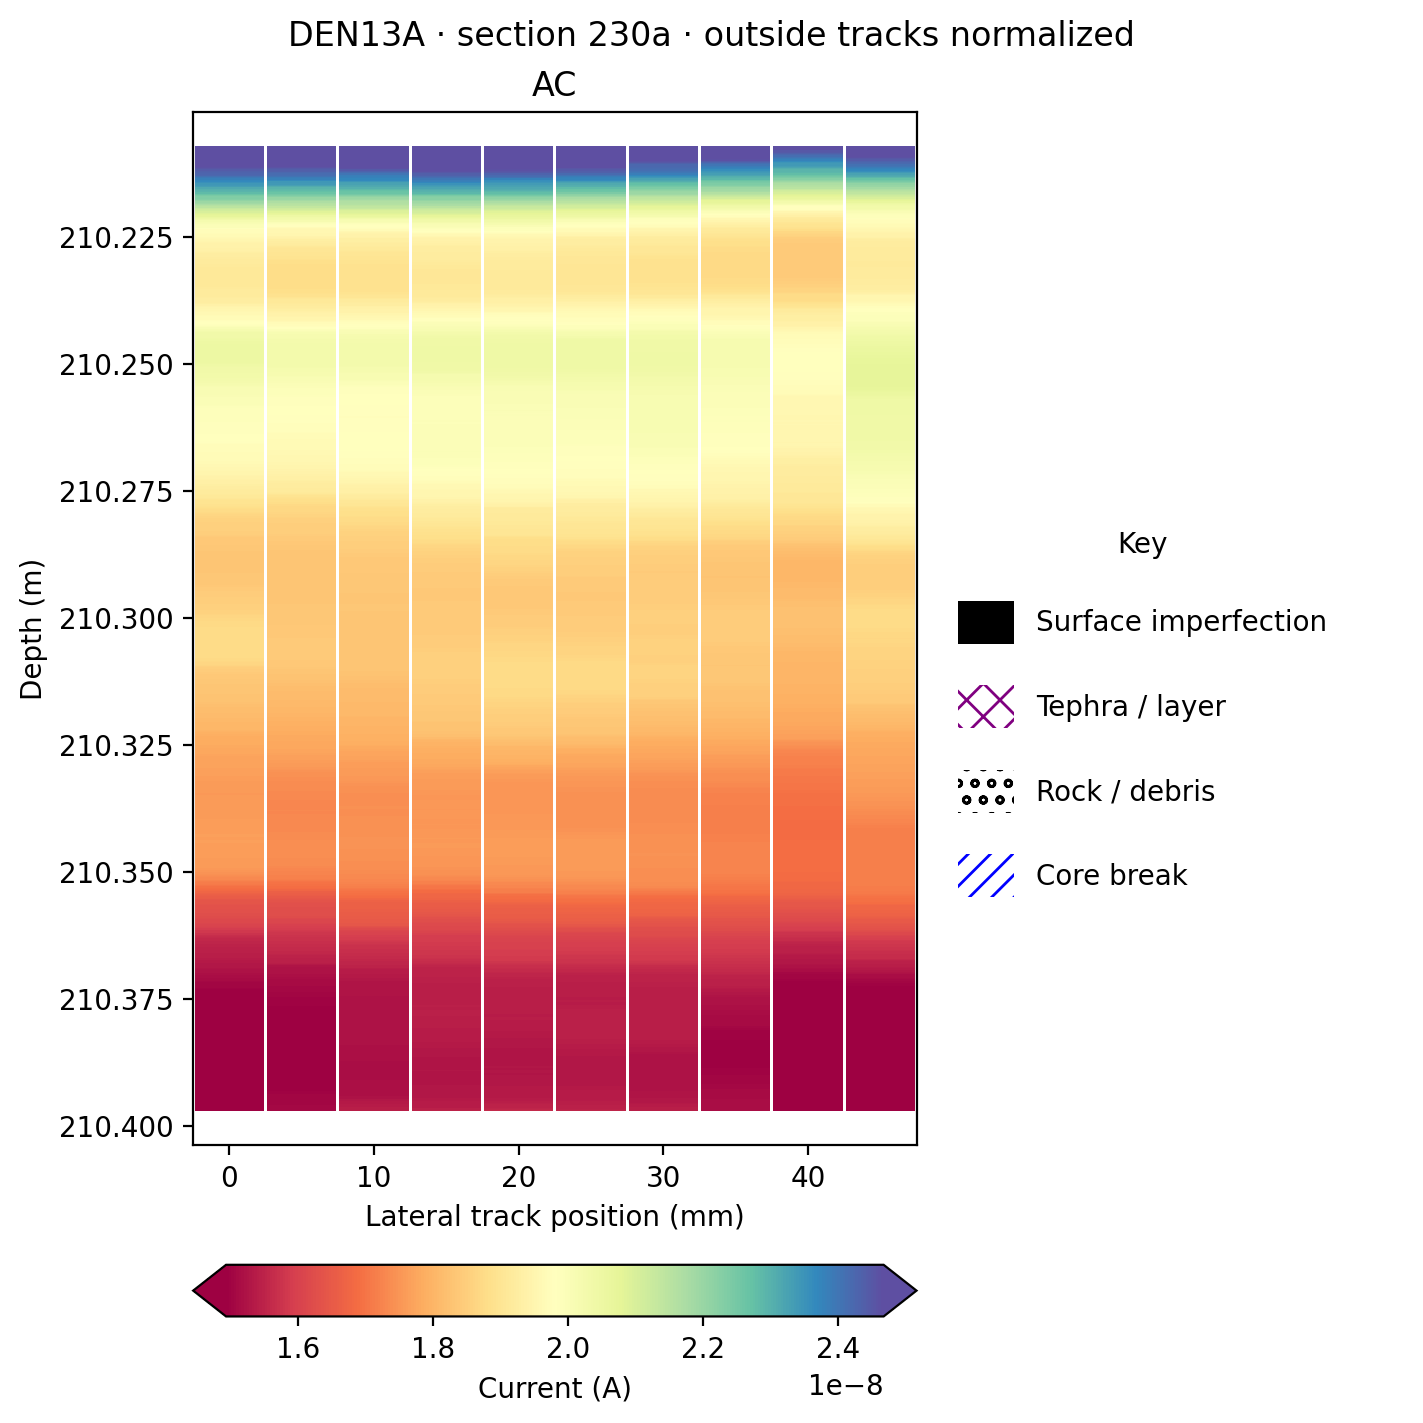
\includegraphics[width=0.72\textwidth]{figures/DEN13A-230a-AC-only.png}
    \caption{AC ECM for section 230a of DEN13A, at approximately 210.20--210.40 m in the displayed map. Broad current variations lack the clear, well-defined layering seen in Fig.~\ref{fig:AC_only_example}. Display processing and annotation conventions are the same as in that figure, with a section-specific color scale.}
    \label{fig:AC_unclear_example}
\end{figure}

The second set of figures includes DC ECM data for the 9 sections (of 16 total) with available DC measurements. AC and DC maps are shown side by side on a shared depth scale, with separate current color scales and the same annotation conventions (Fig.~\ref{fig:AC_and_DC_example}). The other sections' combined plots explicitly indicate the absence of DC data. In section 224abc, corresponding bands are visible in both modes, but the DC map shows greater variation between tracks.

\begin{figure}[H]
    \centering
    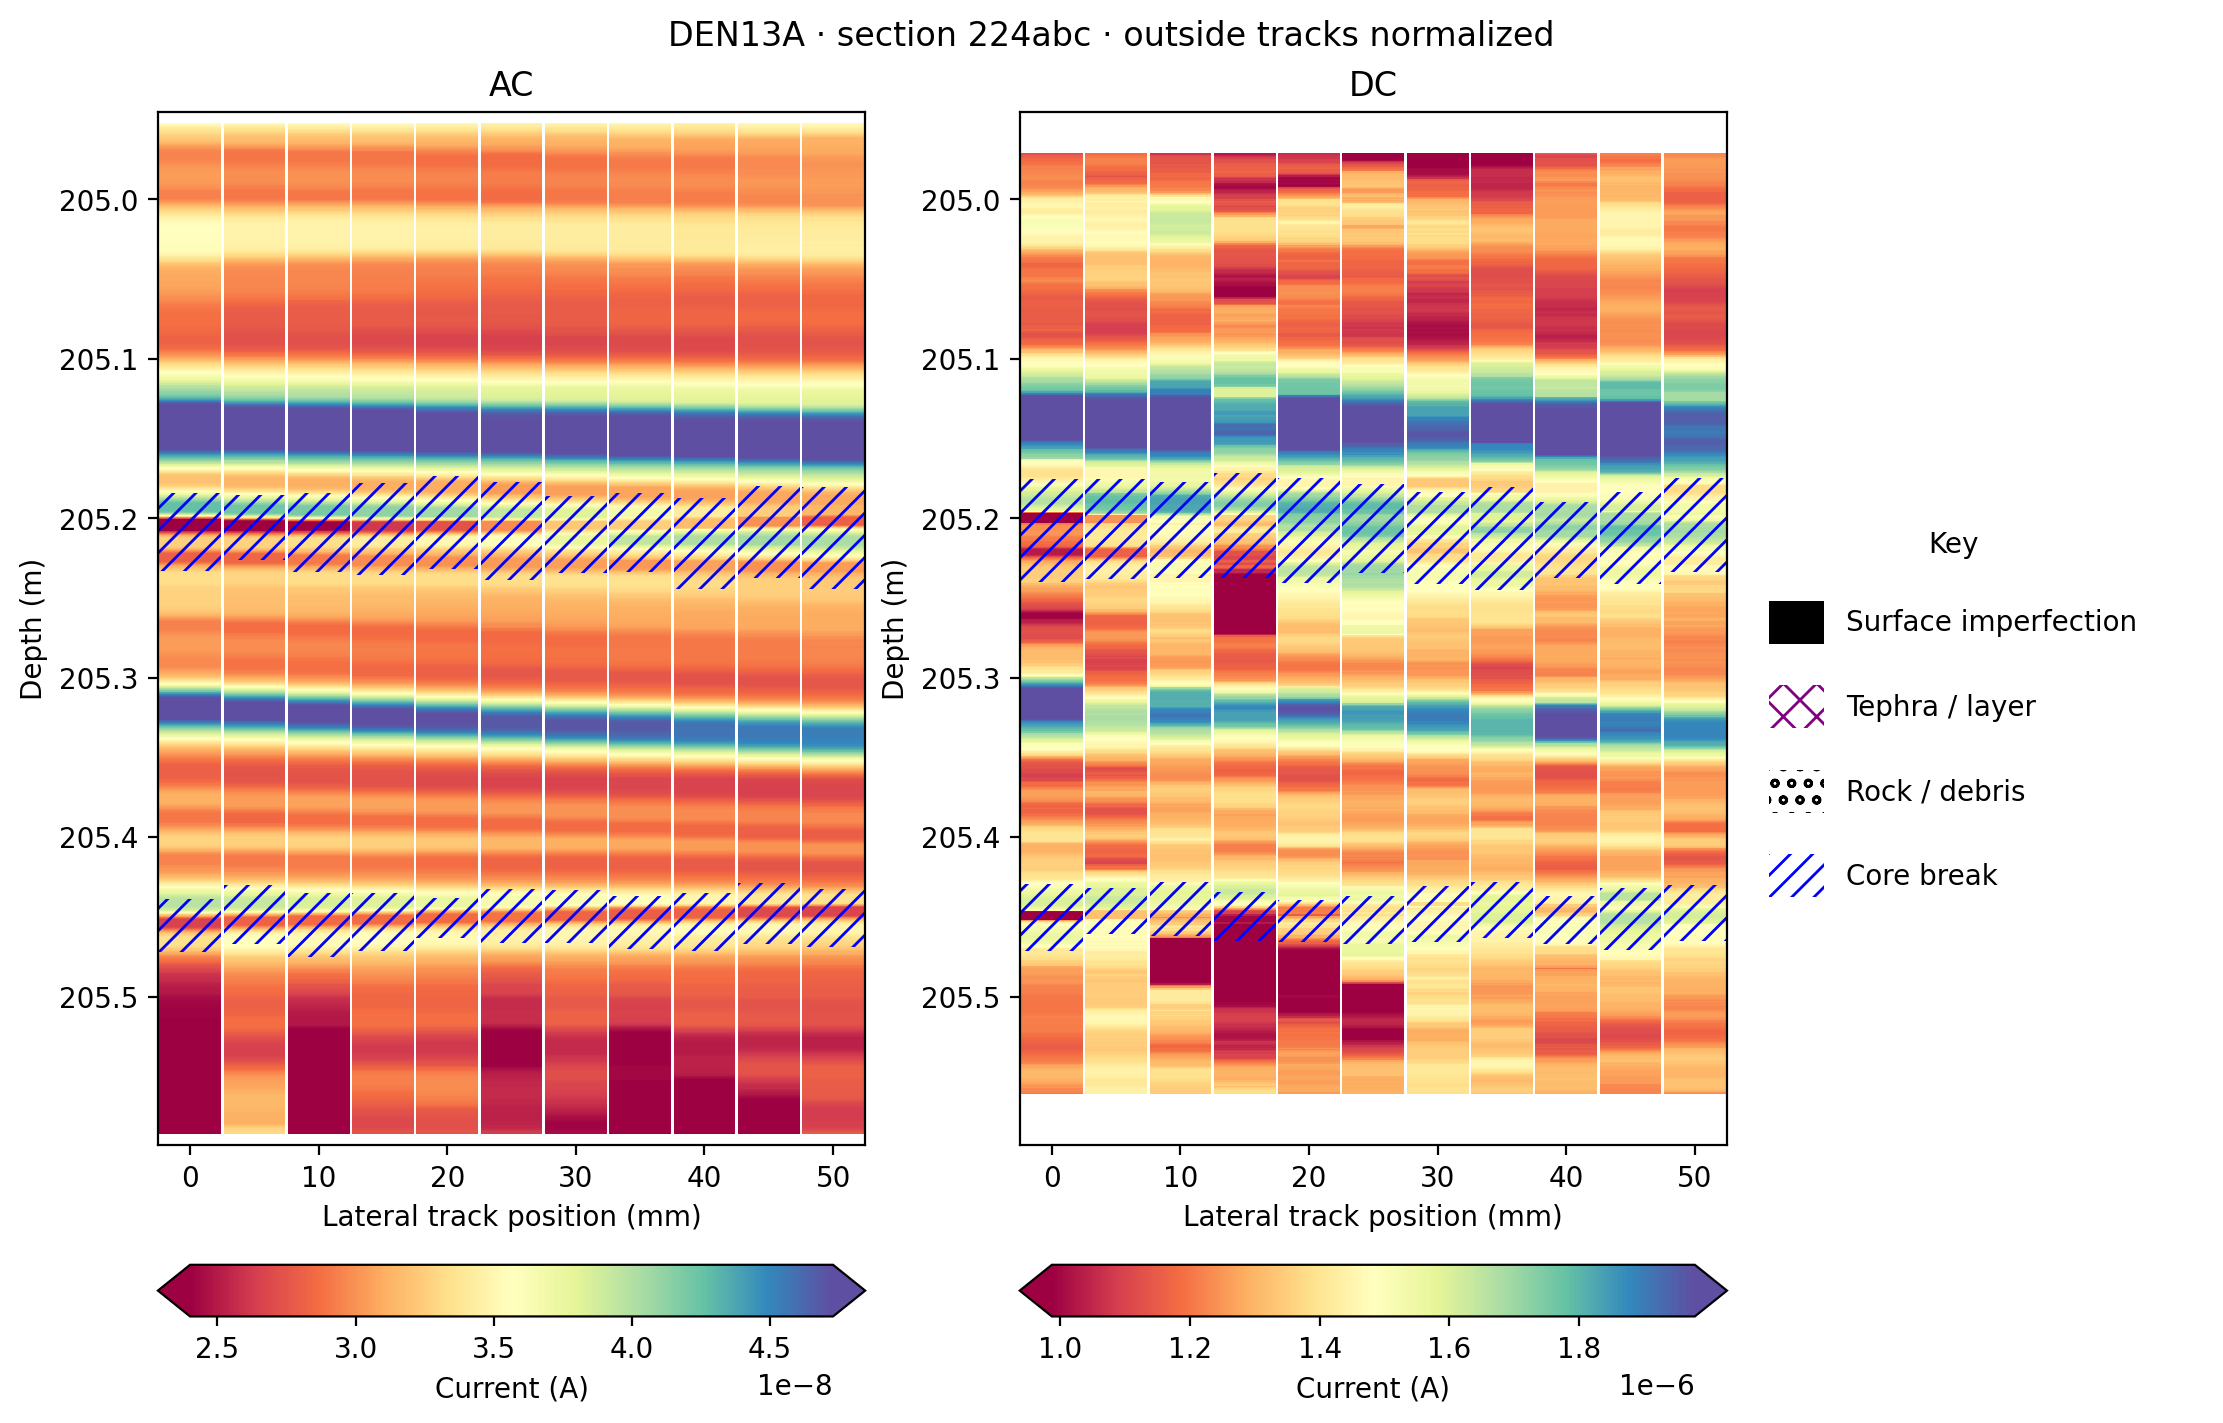
\includegraphics[width=\textwidth]{figures/DEN13A-224abc-AC-and-DC.png}
    \caption{AC (left) and DC (right) ECM for section 224abc of DEN13A. Both maps show recognizable bands, with greater lateral variability in the DC measurements. Each panel has its own current scale; matching colors do not imply equal currents. Blue diagonal hatching indicates core breaks.}
    \label{fig:AC_and_DC_example}
\end{figure}

The third set of figures demonstrates the apparent dip calculation by overlaying individual track extrema and fitted lines on the AC map, alongside the resulting angles and their 95\% confidence intervals (Fig.~\ref{fig:dip_example}). In section 216abcdef, the fit labeled 5 appears to move from the lower edge of a broad layer on the left to its upper edge on the right. This may explain its steeper fitted dip than features 6 and 7 immediately below, whose dip magnitudes are approximately $12^\circ$. It is therefore possible that fit 5 overestimates the inclination of the layer itself.

\begin{figure}[H]
    \centering
    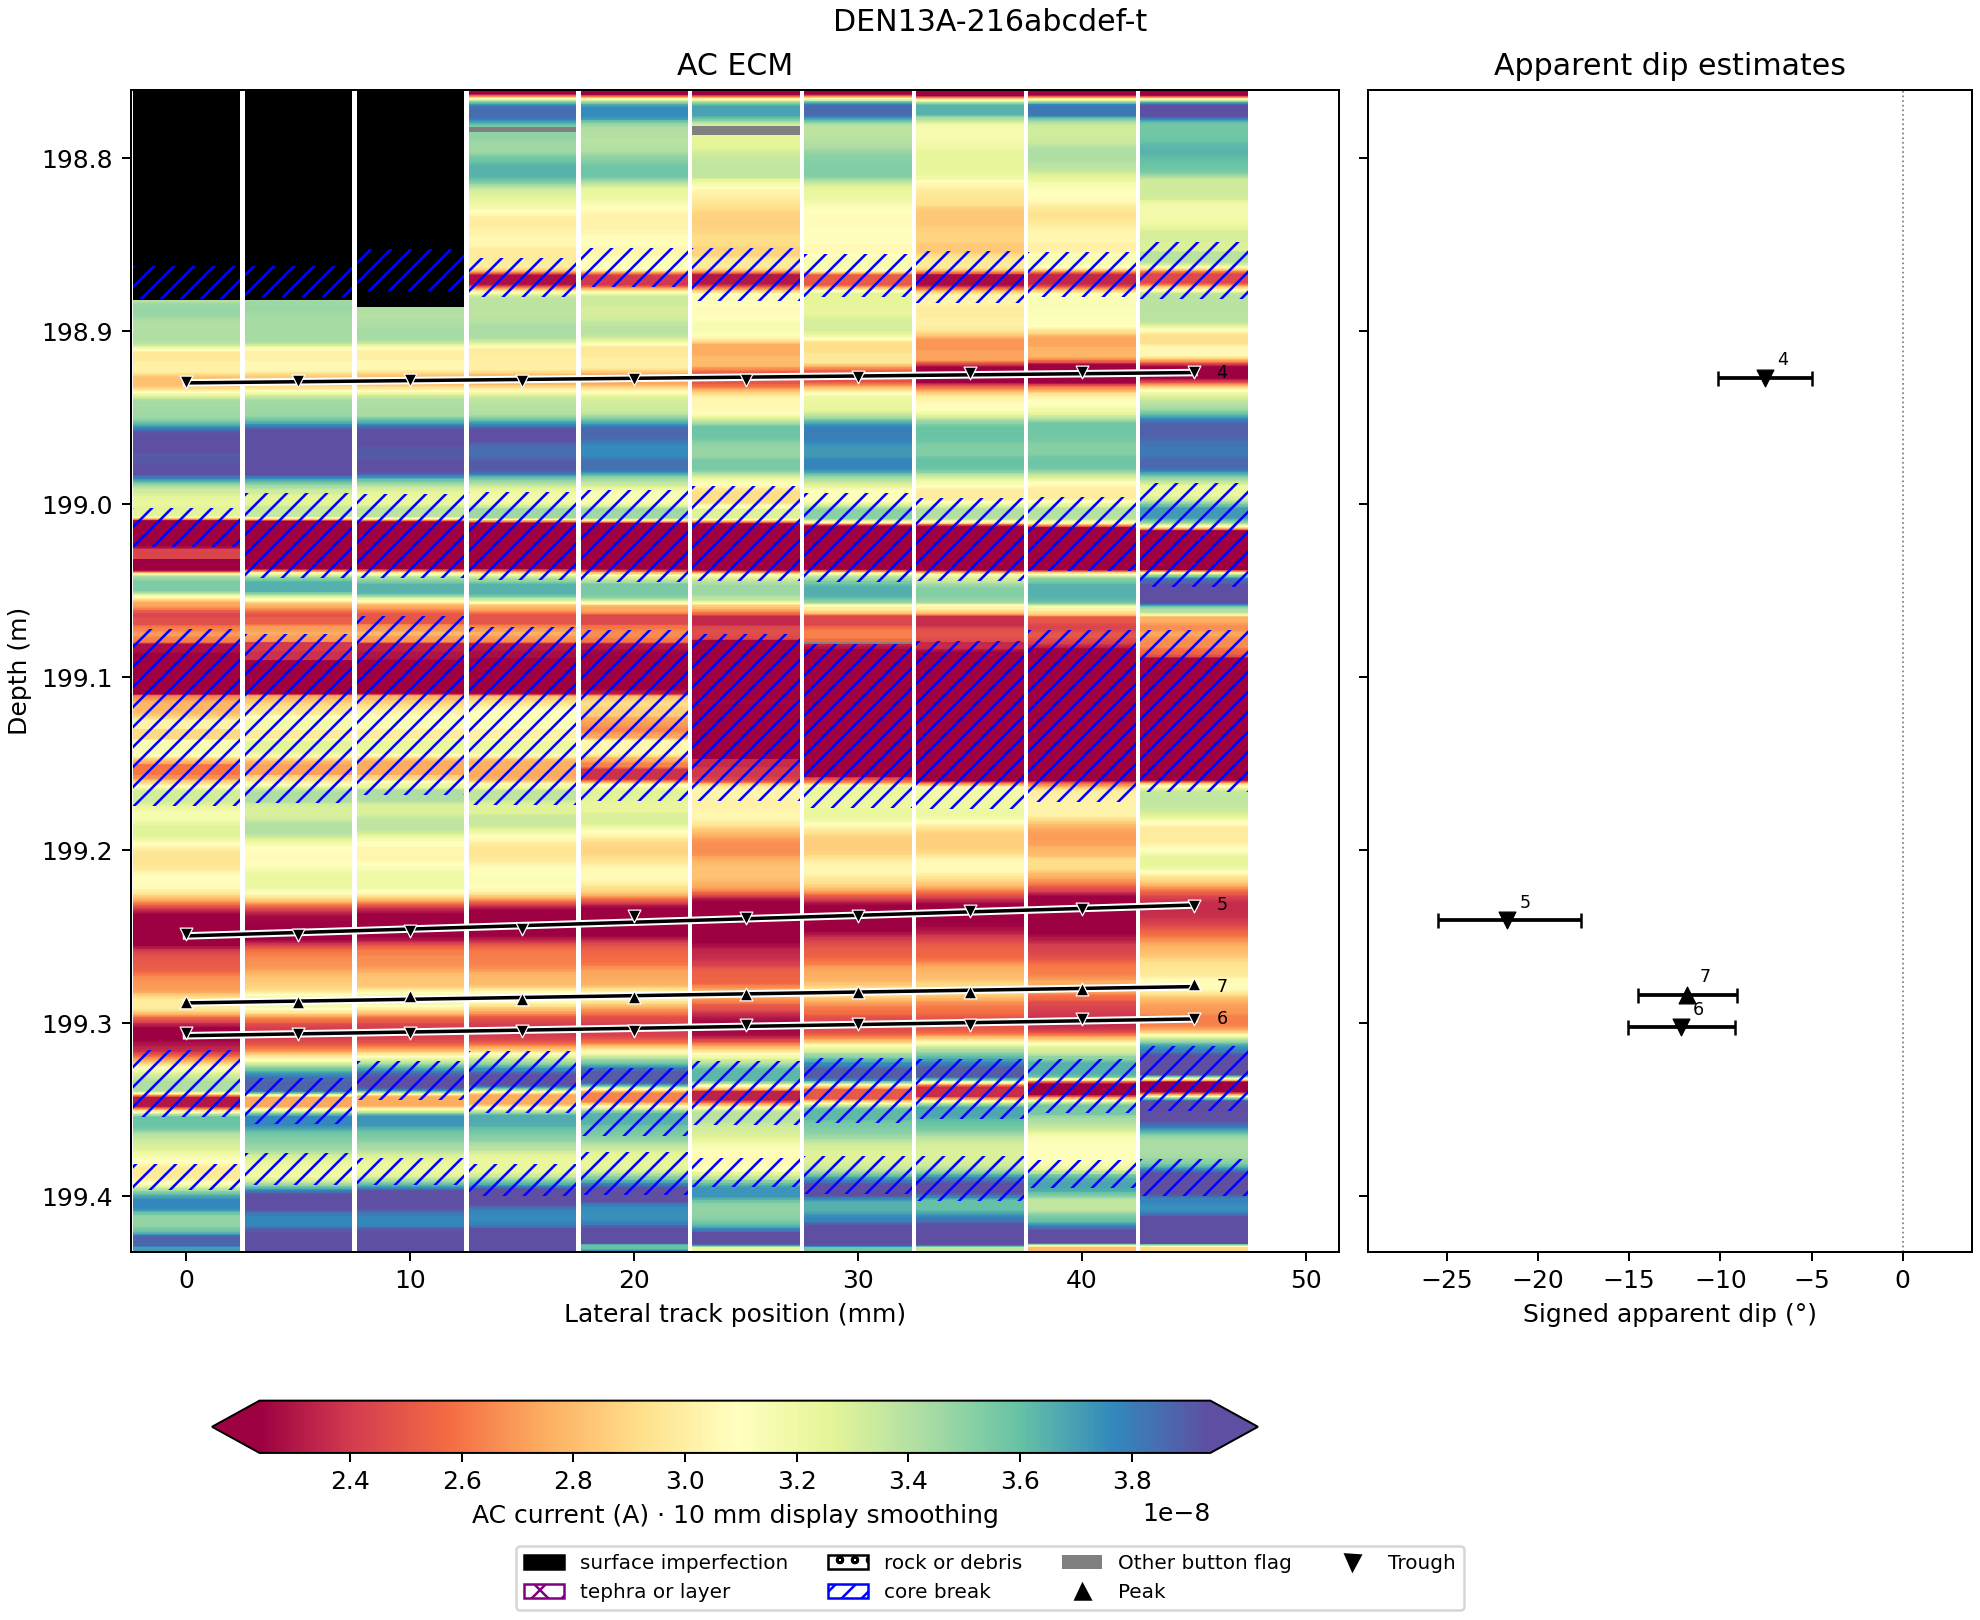
\includegraphics[width=\textwidth]{figures/DEN13A-216abcdef-dips.png}
    \caption{Apparent dip analysis for section 216abcdef of DEN13A. Left: AC current map with raw peak (upward triangles) and trough (downward triangles) picks and fitted lines. Right: signed apparent dip estimates at the mean picked depths, with horizontal 95\% regression confidence intervals. Labels identify the same features in both panels. Fit 5 appears to cross from the lower to the upper part of a broad layer from left to right, potentially inflating its dip magnitude relative to the layers below.}
    \label{fig:dip_example}
\end{figure}

Figure~\ref{fig:dip_over_depth_figure} summarizes all 30 fitted features over depth. Only one point estimate has an apparent dip magnitude exceeding $20^\circ$: fit 5 in section 216abcdef, at approximately 199.24 m, with a signed apparent dip of $-21.7^\circ$ (95\% interval: $-25.5^\circ$ to $-17.6^\circ$). The visual concern described above suggests that this fit may overestimate layer dip. All other point estimates have magnitudes below $20^\circ$, although some confidence intervals extend beyond that threshold. Both positive and negative apparent dips are expected when the core's orientation relative to the measured face changes between sections; such changes need not reflect abrupt changes in the original layer orientation. The numerous core breaks visible within sections also allow relative rotation of individual pieces, so apparent dip can change within a section as well. Overall, the measured apparent dips are generally below $20^\circ$ in magnitude, but these single-face measurements cannot exclude larger true dips. No manual features were fitted below section 227b (deepest fitted feature at 208.25 m); the absence of estimates at greater depths is not evidence of zero dip.

\begin{figure}[H]
    \centering
    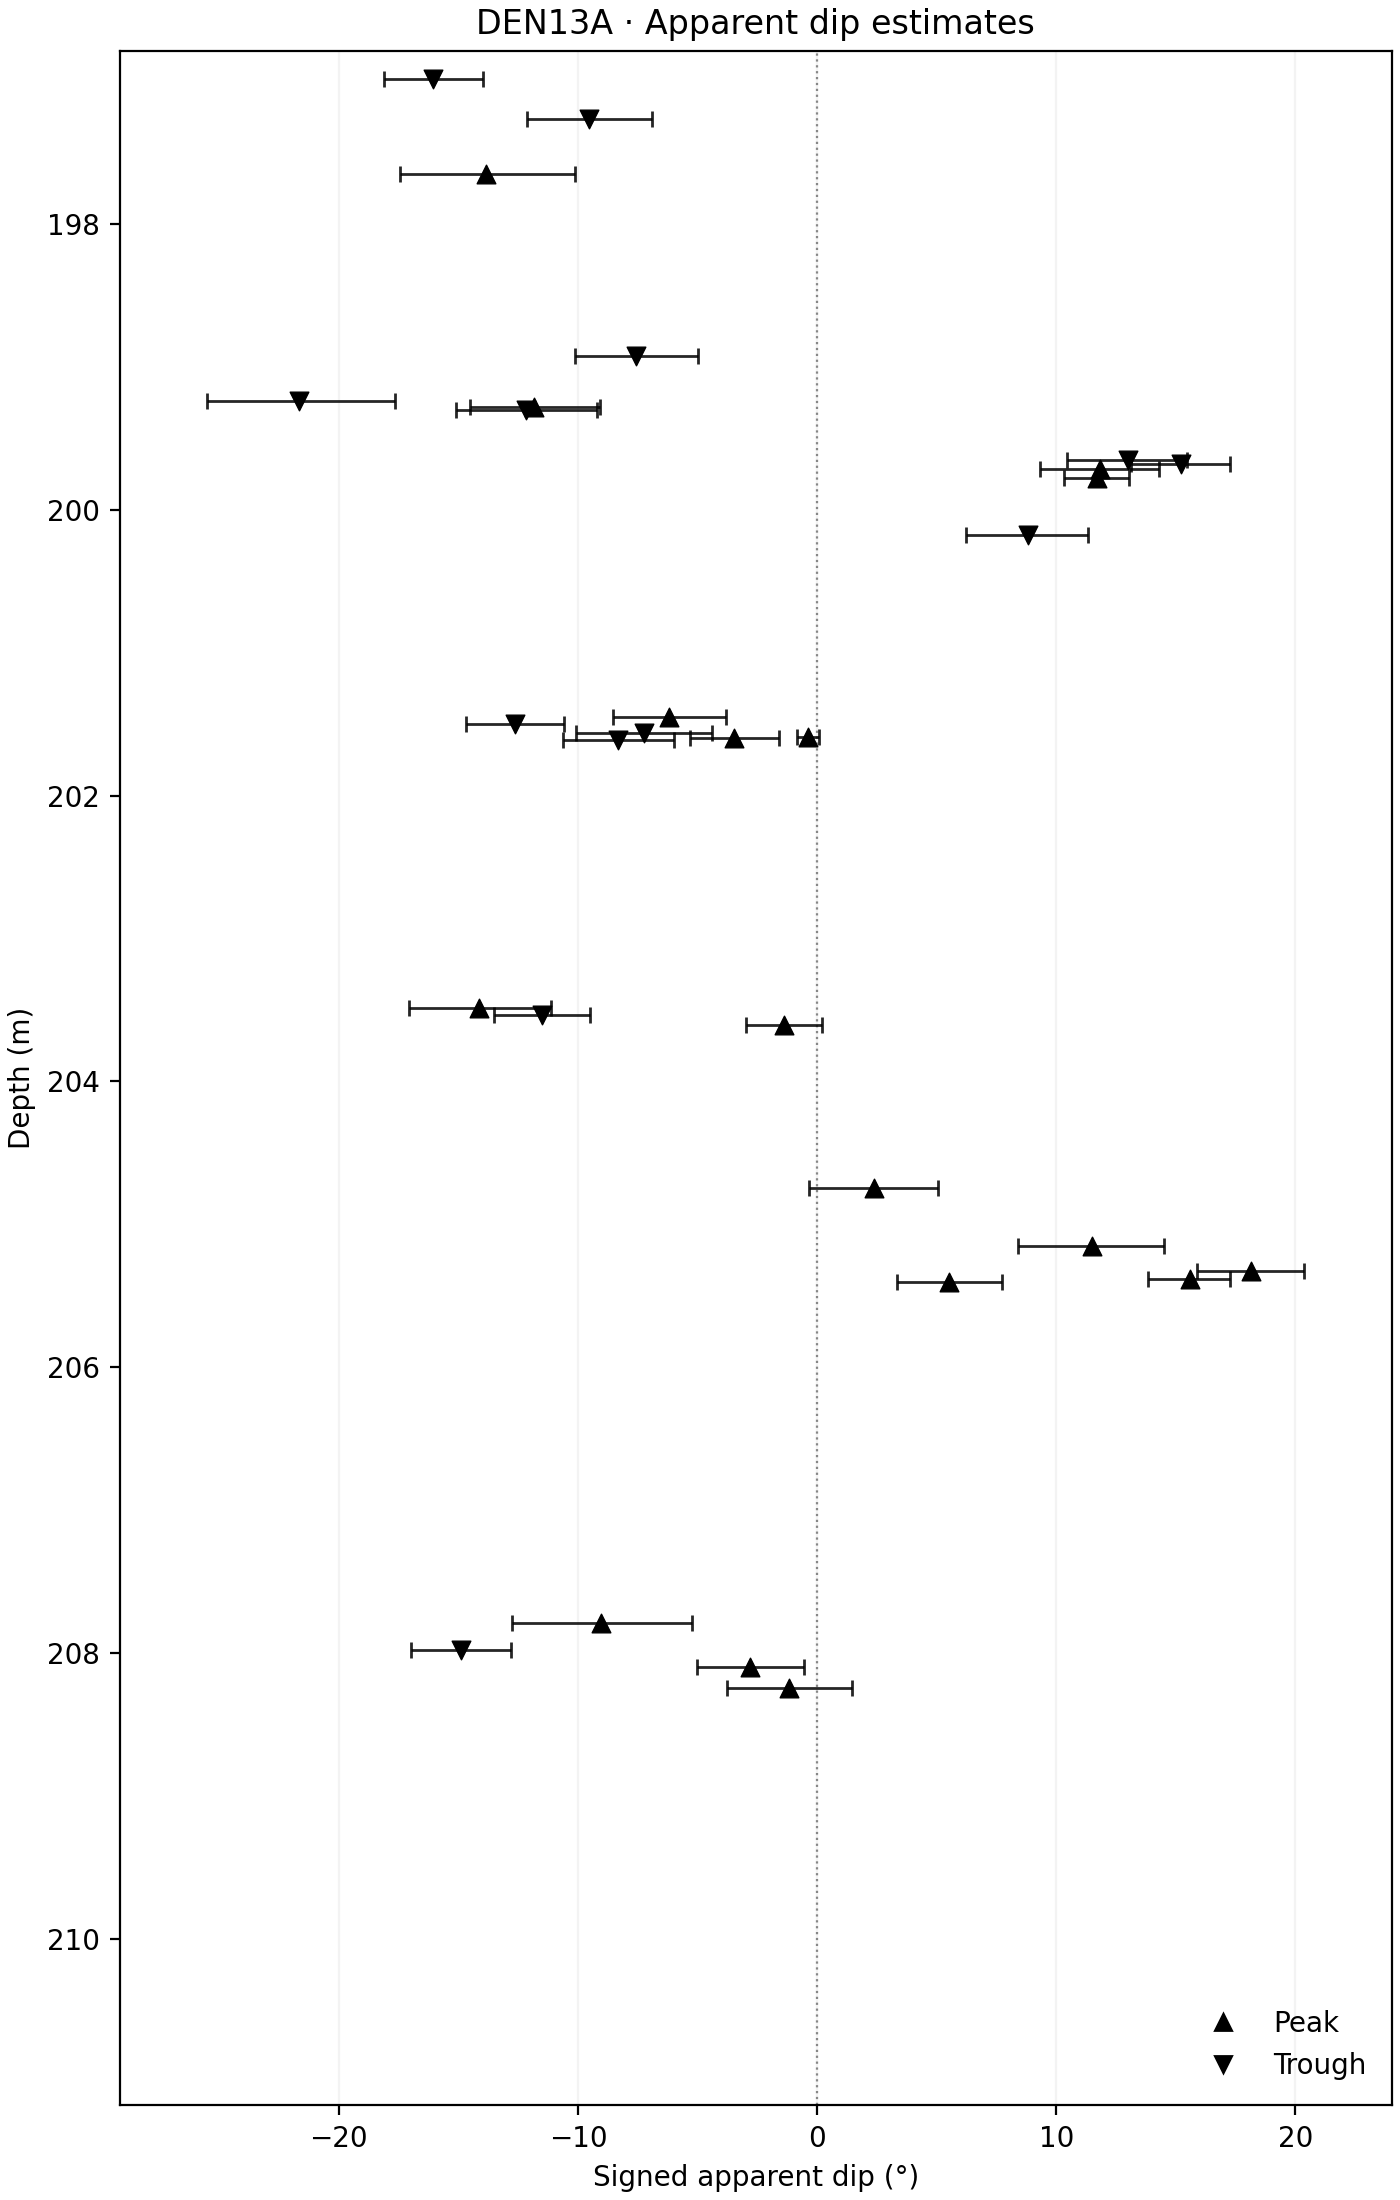
\includegraphics[width=0.68\textwidth,height=0.73\textheight,keepaspectratio]{figures/DEN13A-overall-dips.png}
    \caption{All 30 signed apparent dip estimates for DEN13A on a continuous depth axis. Upward and downward triangles denote peaks and troughs, respectively; horizontal bars show 95\% regression confidence intervals conditional on the picks. Only one point estimate exceeds $20^\circ$ in magnitude, corresponding to fit 5 in Fig.~\ref{fig:dip_example}. Gaps indicate depths without fitted features.}
    \label{fig:dip_over_depth_figure}
\end{figure}

% ============================================
\clearpage
\section{Conclusion}
% ============================================

These results do not provide definitive proof of continuous stratigraphy. However, the measured sections between 196.93 m and approximately 209.14 m provide evidence of recognizable layering that appears locally planar on the measured face, with no visible folding in the clearly resolved layers. Apparent dip magnitudes are generally below $20^\circ$, despite changes in core orientation between sections and potentially across breaks within sections. Larger true dips remain possible because only one face was measured. Deeper sections, including 230a, lack sufficiently clear layering for the same interpretation. Together with independent chronological and stratigraphic evidence, these observations could help evaluate whether the near-basal Denali ice preserves an intact Holocene onset record.

% ============================================
% REFERENCES
% ============================================

\printbibliography[title={References}]


\end{document}
